% Build with two LuaLaTeX passes from docs/manual. Images are relative to this directory.
\documentclass[fontsize=10.2bp,DIV=calc,oneside,open=any,headings=normal,numbers=noenddot]{scrbook}
\usepackage[ngerman]{babel}
\usepackage[a4paper,left=19mm,right=19mm,top=25mm,bottom=24mm,headsep=5mm,footskip=12mm]{geometry}
\usepackage{lmodern,fontspec}
\setmainfont{segoeui.ttf}[
  Path=C:/Windows/Fonts/,BoldFont=segoeuib.ttf,
  ItalicFont=segoeuii.ttf,BoldItalicFont=segoeuiz.ttf
]
\renewcommand{\sfdefault}{\rmdefault}
\setmonofont{consola.ttf}[
  Path=C:/Windows/Fonts/,BoldFont=consolab.ttf,
  ItalicFont=consolai.ttf,BoldItalicFont=consolaz.ttf
]
\usepackage[table]{xcolor}
\usepackage{microtype,graphicx,float,caption}
\usepackage{scrlayer-scrpage}
\usepackage{booktabs,tabularx,array,needspace,fvextra,xurl}
\usepackage{hyperref,bookmark}

\definecolor{Ink}{HTML}{142E46}
\definecolor{Teal}{HTML}{00857D}
\definecolor{Muted}{HTML}{526171}
\definecolor{Rule}{HTML}{CBD8E0}
\newcommand{\ProductName}{6502 SBC Emulator}
\newcommand{\ManualTitle}{Bedienung und Konfiguration}
\newcommand{\ManualDate}{21. November 2026}
\newcommand{\ui}[1]{\textbf{#1}}
\newcommand{\metaSize}{\fontsize{8bp}{10bp}\selectfont}
\newcommand{\tableSize}{\fontsize{9bp}{11bp}\selectfont}
\newcommand{\captionSize}{\fontsize{8.6bp}{11bp}\selectfont}
\newcolumntype{Y}{>{\raggedright\arraybackslash}X}
\newcolumntype{P}[1]{>{\raggedright\arraybackslash}p{#1}}

\hypersetup{
  colorlinks=true,linkcolor=Teal,urlcolor=Teal,
  pdftitle={6502 SBC Emulator - Bedienung und Konfiguration},
  pdfauthor={Rudolf Stepan},pdfsubject={Deutschsprachiges Emulator-Handbuch},
  pdflang=de-DE,bookmarksdepth=1
}
\setlength{\parindent}{0pt}
\setlength{\parskip}{5.2pt plus 1pt minus 1pt}
\setlength{\emergencystretch}{3em}
\linespread{1.08}
\widowpenalty=10000
\clubpenalty=10000
\raggedbottom
\raggedright
\color{Ink}
\setkomafont{disposition}{\sffamily\bfseries\color{Ink}}
\setkomafont{chapter}{\fontsize{24bp}{29bp}\selectfont}
\setkomafont{section}{\fontsize{15bp}{18bp}\selectfont\color{Teal}}
\setkomafont{subsection}{\fontsize{11.5bp}{14bp}\selectfont}
\RedeclareSectionCommand[beforeskip=0pt,afterskip=16pt]{chapter}
\RedeclareSectionCommand[beforeskip=-14pt plus -2pt minus -1pt,afterskip=5pt]{section}
\setcounter{tocdepth}{1}
\setcounter{secnumdepth}{1}
\DeclareTOCStyleEntries[entryformat=\tableSize,pagenumberformat=\tableSize,
  pagenumberwidth=2.2em]{tocline}{section,figure}
\DeclareTOCStyleEntry[pagenumberformat=\tableSize,pagenumberwidth=2.2em]{tocline}{chapter}

\clearpairofpagestyles
\automark[chapter]{chapter}
\ihead*{\textcolor{Teal}{\textbf{\ProductName}}}
\ohead*{\headmark}
\ifoot*{\ManualTitle\enspace|\enspace Deutsch\enspace|\enspace\ManualDate}
\ofoot*{Seite\nobreakspace\pagemark}
\KOMAoptions{headsepline=0.4pt:head,plainheadsepline}
\setkomafont{pageheadfoot}{\sffamily\metaSize\color{Muted}}
\setkomafont{headsepline}{\color{Rule}}
\pagestyle{scrheadings}

\DeclareCaptionFont{manual}{\captionSize}
\captionsetup{font={manual,sf,color=Muted},labelfont=bf,labelsep=period,
  justification=raggedright,singlelinecheck=false,skip=5pt}
\counterwithout{figure}{chapter}
\newcommand{\shot}[3]{%
  \begin{figure}[H]
    \centering
    \begin{minipage}{#1}
      \includegraphics[width=\linewidth]{screenshots/#2.png}
      \caption{#3}
    \end{minipage}
  \end{figure}%
}
\renewcommand{\arraystretch}{1.16}
\setlength{\tabcolsep}{5pt}
\NewDocumentEnvironment{referenceTable}{m +b}{%
  \begin{minipage}{\linewidth}\tableSize
    \arrayrulecolor{Rule}%
    \begin{tabularx}{\linewidth}{@{}#1@{}}
      \toprule
      #2
      \bottomrule
    \end{tabularx}
  \end{minipage}
}{}
\fvset{fontsize=\tableSize,frame=leftline,rulecolor=\color{Rule},
  framesep=6pt,xleftmargin=8pt,breaklines=true,samepage=true}
\DefineVerbatimEnvironment{commandblock}{Verbatim}{}

\begin{document}
\hypersetup{pageanchor=false}
\begin{titlepage}
  \sffamily
  \vspace*{14mm}
  {\color{Teal}\bfseries\fontsize{23bp}{27bp}\selectfont\ProductName\par}
  \vspace{8mm}
  {\color{Ink}\bfseries\fontsize{33bp}{38bp}\selectfont\ManualTitle\par}
  \vspace{7mm}
  {\color{Teal}\fontsize{17bp}{22bp}\selectfont SBC und Commodore 64 (PAL)\par}
  \vspace{10mm}
  \noindent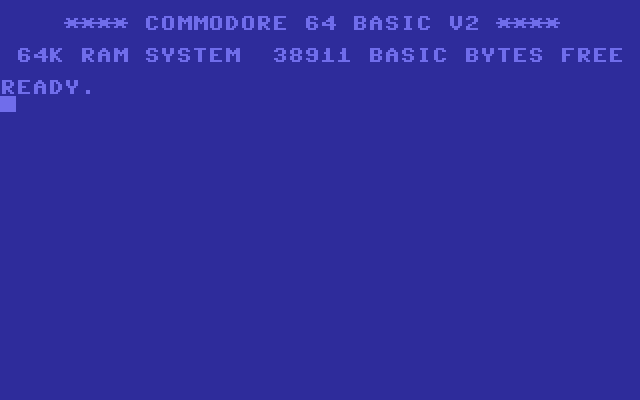
\includegraphics[width=\linewidth]{screenshots/c64-start.png}\par
  {\captionSize\color{Muted}C64-BASIC mit geladenen ROMs und Eingabeprompt.\par}
  \vfill
  \noindent\textcolor{Rule}{\rule{\linewidth}{0.5pt}}\par
  \begin{minipage}[t]{.46\linewidth}
    \captionSize\textbf{Rudolf Stepan}\par
    Deutschsprachiges Bedienhandbuch
  \end{minipage}\hfill
  \begin{minipage}[t]{.5\linewidth}
    \raggedleft\captionSize\color{Muted}
    Lokaler Windows-Build\par
    Dokumentationsstand \ManualDate
  \end{minipage}
\end{titlepage}

\frontmatter
\hypersetup{pageanchor=true}
\tableofcontents
\vspace{12pt}
\textbf{Schneller Einstieg.} Starten Sie den C64 wie in Kapitel~\ref{ch:start}
beschrieben. Der erste Prüfbefehl erzeugt die Ausgabe \texttt{42}. Kapitel~\ref{ch:menu}
beschreibt das F12-Menü. Mit Kapitel~\ref{ch:disk} legen Sie eine virtuelle Diskette ein.

\mainmatter
\chapter{Start und erster Test}\label{ch:start}

\section{Windows-Build und Profil}
Der Emulator bietet ein SBC-Profil mit eigenen ROMs und ein PAL-C64-Profil mit
separaten C64-ROMs. Beim Start bestimmt die gewählte INI-Datei die Maschine und
ihre Einstellungen. Dieser Leitfaden beschreibt den lokalen Build vom
\ManualDate. Die Abbildungen stammen aus der gerenderten Programmoberfläche.

\section{C64-ROMs bereitstellen}
Der C64-Start benötigt drei lokal bereitgestellte ROM-Dateien. Legen Sie sie
unter \path{roms/c64/} im Projektordner ab. Die Dateinamen entsprechen den
Vorgaben in \path{c64.ini}.

\begin{referenceTable}{l l Y}
\textbf{ROM} & \textbf{Dateiname} & \textbf{Größe} \\
\midrule
BASIC & \texttt{basic.rom} & 8192 Byte \\
KERNAL & \texttt{kernal.rom} & 8192 Byte \\
Zeichengenerator & \texttt{chargen.rom} & 4096 Byte \\
\end{referenceTable}

\section{BASIC-Prompt prüfen}
\begin{enumerate}
  \item Starten Sie \path{Start-C64.bat} im Projektordner. Die Batchdatei
    startet \path{bin/sbc6502.exe} mit der \path{c64.ini} aus dem Projektordner.
  \item Warten Sie auf \texttt{READY.} und klicken Sie bei Bedarf in das C64-Fenster.
  \item Geben Sie den folgenden Befehl ein und drücken Sie \ui{Enter}.
\end{enumerate}

\begin{commandblock}
PRINT 7*6
\end{commandblock}
\textbf{Erwartetes Ergebnis.} BASIC zeigt \texttt{42} an und kehrt zu
\texttt{READY.} zurück. Je nach PC-Belegung erreichen Sie das C64-Sternchen
über \ui{*} auf dem Ziffernblock.

\section{Start über PowerShell}
Aus dem Projektordner können Sie das gleiche Profil direkt aufrufen.
Relative Pfade in der INI werden aus dem Arbeitsverzeichnis aufgelöst.

\begin{commandblock}
.\bin\sbc6502.exe c64.ini
\end{commandblock}

\chapter{Konfigurationsmenü}\label{ch:menu}

\section{Einstellungen ändern und speichern}
Drücken Sie im C64-Fenster \ui{F12}. Die Emulation pausiert und das Menü öffnet
die zuletzt gewählte Seite. Beim ersten Aufruf erscheint \ui{SETTINGS}.

\shot{127mm}{c64-settings}{\ui{SETTINGS} mit Fensterzoom, CPU-Takt, Floppy und ROM-Pfaden.}

\begin{referenceTable}{P{43mm} Y}
\textbf{Taste} & \textbf{Funktion im Menü} \\
\midrule
\ui{Tab} / \ui{Umschalt+Tab} & Seite vorwärts oder rückwärts wechseln. \\
\ui{Pfeil auf} / \ui{Pfeil ab} & Eintrag wählen. \ui{Bild auf} und \ui{Bild ab} springen seitenweise. \\
\ui{Pfeil links} / \ui{Pfeil rechts} & Numerischen Wert oder Auswahl ändern. \\
\ui{Enter} & Eintrag bearbeiten oder eine neue Eingabe für die Belegung erfassen. \\
\ui{Entf} & Ausgewählte Tasten- oder Controllerbelegung auf den Standard zurücksetzen. \\
\ui{F2} & Speichern und das Menü geöffnet lassen. \\
\ui{F12} & Menü schließen, ungespeicherte Änderungen verwerfen und die Emulation fortsetzen. \\
\end{referenceTable}

\section{Sofortige und spätere Wirkung}
Der Zoom und die Eingabebelegungen gelten nach \ui{F2} sofort. Einstellungen
mit Stern, etwa \ui{CPU SPEED HZ}, \ui{START IMAGE} und die ROM-Pfade, werden
beim nächsten Emulatorstart übernommen. Bestätigen Sie eine Texteingabe mit
\ui{Enter}, bevor Sie speichern.

\chapter{Tastatur und Joystick}\label{ch:input}

\section{C64-Tastatur belegen}
Öffnen Sie mit \ui{F12} das Menü und wechseln Sie mit \ui{Tab} zu \ui{KEYBOARD}.

\shot{116mm}{c64-keyboard}{\ui{KEYBOARD} zeigt die emulierte Taste links und die PC-Taste rechts.}

\begin{enumerate}
  \item Wählen Sie eine C64-Taste, beispielsweise \ui{INST/DEL} oder \ui{RUN/STOP}.
  \item Drücken Sie \ui{Enter} und dann die gewünschte PC-Taste.
  \item Speichern Sie mit \ui{F2}. Schließen Sie das Menü mit \ui{F12} und
    prüfen Sie die neue Belegung im C64-Programm.
\end{enumerate}

\begin{referenceTable}{P{52mm} Y}
\textbf{PC-Taste in der Standardbelegung} & \textbf{C64-Funktion} \\
\midrule
\ui{Escape} oder \ui{Tab} & \ui{RUN/STOP} im laufenden C64-Profil \\
\ui{Bild auf} & \ui{RESTORE} \\
\ui{Rücktaste} oder \ui{Entf} & \ui{INST/DEL} \\
\ui{Alt} & Commodore-Taste \\
\ui{Pfeiltasten} & Cursor, sofern die PC-Tasten nicht dem aktiven Joystick zugeordnet sind \\
\end{referenceTable}

\textbf{Fenster schließen.} Im C64-Profil beendet die Fenster-Schaltfläche
den Emulator. \ui{Escape} wird an die emulierte Tastatur weitergegeben.

\clearpage
\section{Joystick-Port und Eingabegerät}\label{sec:joystick}
Auf der Seite \ui{JOYSTICK} steuert die erste Zeile den emulierten Port.
Wählen Sie \ui{PORT 1} oder \ui{PORT 2} passend zum Programm. \ui{OFF}
deaktiviert die Joystick-Eingaben.

\shot{127mm}{c64-joystick}{\ui{JOYSTICK} mit Portwahl und getrennten Belegungen für Tastatur und USB-Controller.}

\begin{enumerate}
  \item Wählen Sie für eine PC-Taste eine Zeile \ui{KEY UP} bis \ui{KEY FIRE}.
    Drücken Sie \ui{Enter} und dann die gewünschte Taste.
  \item Für einen USB-Joystick oder ein Gamepad wählen Sie eine Zeile
    \ui{PAD UP} bis \ui{PAD FIRE}. Drücken Sie \ui{Enter} und bewegen Sie die
    Achse, betätigen Sie das Steuerkreuz oder drücken Sie die gewünschte Taste.
  \item Speichern Sie mit \ui{F2} und kehren Sie mit \ui{F12} zum Programm zurück.
\end{enumerate}

\section{Standardbelegung und Kontrolle}
Bei aktiviertem Port verwenden die Standardbelegungen der Tastatur die
Pfeiltasten für die Richtung und \ui{Strg rechts} für Feuer. Für USB-Eingaben
verwendet der Emulator das erste von SDL geöffnete Gerät. Bei \ui{AUTO}
liefern die ersten beiden Achsen oder das erste Steuerkreuz die Richtungen.
Die erste Taste liefert Feuer.

Ist eine PC-Taste dem Joystick zugeordnet, wird sie im laufenden C64-Profil
als Joystick-Eingabe ausgewertet. Wenn Sie die Pfeiltasten für den BASIC-Cursor
benötigen, weisen Sie dem Joystick andere PC-Tasten zu oder wählen Sie \ui{OFF}.

\chapter{Disketten und Programme}\label{ch:disk}

\section{D64 einlegen und Verzeichnis anzeigen}
Voraussetzung ist ein 35-Spur-D64-Abbild und ein laufendes C64-Profil.
Das virtuelle Laufwerk liest das Abbild schreibgeschützt.

\begin{enumerate}
  \item Ziehen Sie die \path{.d64}-Datei auf das C64-Fenster. Im Titel erscheinen
    die Gerätenummer und der Dateiname.
  \item Geben Sie im BASIC-Prompt die folgenden Befehle ein. Ersetzen Sie
    \texttt{8}, wenn in \ui{FLOPPY DEVICE} ein anderes Gerät eingestellt ist.
\end{enumerate}

\begin{commandblock}
LOAD "$",8
LIST
\end{commandblock}
\textbf{Erwartetes Ergebnis.} \texttt{LIST} zeigt den Diskettennamen und die
Dateieinträge. Der Verzeichnis-\texttt{LOAD} ersetzt das aktuell im
BASIC-Speicher liegende Programm.

\section{PRG laden und starten}
Benutzen Sie den Namen zwischen den Anführungszeichen im Verzeichnis. Ohne
Sekundäradresse lädt BASIC ein Programm an seinen Standardstart. Mit
\texttt{,1} verwendet der Loader die im PRG gespeicherte Ladeadresse.

\begin{commandblock}
LOAD "NAME",8
RUN
\end{commandblock}

Das erste PRG auf einer Diskette laden Sie mit \texttt{LOAD "*",8,1} an seine
gespeicherte Adresse. \texttt{RUN} startet PRGs mit einem BASIC-Einstieg.
Bei reinen Maschinenprogrammen gilt der dokumentierte Einstieg des Programms.

\section{Startdiskette festlegen}
Öffnen Sie \ui{SETTINGS} im F12-Menü. Bearbeiten Sie \ui{START IMAGE} mit
\ui{Enter} oder ziehen Sie ein D64 auf das geöffnete Menü. Ein leeres Feld
lässt das Laufwerk beim Start leer. Speichern Sie mit \ui{F2} und starten Sie
das C64-Profil erneut. Bei geschlossenem Menü legt Drag-and-drop die Diskette
sofort ein.

\begin{commandblock}
[floppy]
device = 8
image = data/sdcard/example.d64
\end{commandblock}

\chapter{SBC-Modus}\label{ch:sbc}

\section{Ein Profil starten}
Starten Sie SBC-Profile aus dem Projektordner mit ihrem INI-Dateinamen. Das
folgende Beispiel startet das eigenständige Schach-ROM.

\begin{commandblock}
.\bin\sbc6502.exe chess.ini
\end{commandblock}

\shot{116mm}{sbc-schach}{Das Schach-ROM im SBC-Modus.}

\begin{referenceTable}{P{39mm} Y}
\textbf{Profil} & \textbf{Verwendung} \\
\midrule
\path{sbc.ini} & SBC-Kernel mit MS BASIC \\
\path{ehbasic.ini} & SBC-Kernel mit EhBASIC \\
\path{chess.ini} & Eigenständiges Schach-ROM \\
\path{soundtest.ini} & Eigenständige Vierstimmen-Klangdemo \\
\path{avdemo.ini} & Audio- und Videodemo \\
\path{fpga.ini} & FPGA-kompatibles Profil mit geteiltem Shadow-ROM \\
\end{referenceTable}

\section{Bedienung und Konfiguration}
\ui{Escape} oder das Schließen des Fensters beendet die SBC-Emulation. Ändern
Sie SBC-Einstellungen in der verwendeten INI. Der C64-Programmlader für D64
gehört zum C64-Profil. Das FPGA-Profil enthält einen eigenen GoDrive-Ablauf für
Disks unter \path{data/sdcard/}.

\chapter{Konfigurationsreferenz}\label{ch:ref}

\section{Welche INI wird gespeichert?}
\path{Start-C64.bat} liest und speichert die \path{c64.ini} im Projektordner.
Bei einem Direktstart mit einer anderen INI speichert \ui{F2} in dieser
Datei. Wenn Sie \texttt{sbc6502.exe c64.ini} aus \path{bin/} aufrufen, gilt die
Kopie in diesem Verzeichnis. \texttt{make} legt die Projektprofile im
Build-Bundle ab.

\begin{referenceTable}{P{43mm} Y}
\textbf{INI-Feld} & \textbf{Bedeutung im C64-Profil} \\
\midrule
\texttt{[video] window\_scale} & Ganzzahliger Fensterzoom. \texttt{1} öffnet
640 × 400, \texttt{2} öffnet 1280 × 800. Zulässig sind Werte von 1 bis 25. \\
\texttt{[cpu] speed\_hz} & Zielrate in Hz. PAL-Vorgabe \texttt{985248},
\texttt{0} schaltet die Geschwindigkeitsbegrenzung aus. \\
\texttt{[machine]} & \texttt{type = c64}, Pfade für \texttt{basic},
\texttt{kernal} und \texttt{chargen}. \\
\texttt{[floppy]} & \texttt{device} von 8 bis 11 und optionales D64-\texttt{image}. \\
\texttt{[keyboard]} & Überschriebene PC-Scancodes für Tastaturmatrix und \ui{RESTORE}. \\
\texttt{[joystick]} & \texttt{port} sowie zugewiesene PC-Scancodes und Controller-Eingaben. \\
\end{referenceTable}

\section{Build und Diagnose}
Für einen lokalen Windows-Build benötigt das Projekt GNU Make, GCC/MinGW und
die SDL2-Entwicklungsdateien. Führen Sie die Befehle im Projektordner aus.
\texttt{make} legt Programmdatei, Laufzeitdateien und Profile unter \path{bin/} ab.

\begin{commandblock}
make
make test-c64
.\build\test_c64.exe --boot
\end{commandblock}

Der letzte Befehl verwendet die lokalen C64-ROMs und prüft BASIC-Start,
Tastatureingaben, D64-Verzeichnis und PRG-Start. \texttt{-h} zeigt die
Aufrufoptionen. \texttt{-m} zeigt die Speicherbelegung und beendet das Programm.

\chapter{Fehlerdiagnose}\label{ch:trouble}

\section{Start, Bild und Eingaben}
\begin{referenceTable}{P{48mm} Y}
\textbf{Symptom} & \textbf{Prüfen und beheben} \\
\midrule
Beim Start erscheint kein C64-Fenster. & Starten Sie \path{Start-C64.bat} im
Projektordner. Prüfen Sie die Konsolenausgabe und die drei ROM-Dateien anhand
der Größen in Kapitel~\ref{ch:start}. \\
Der geänderte Zoom fehlt. & Prüfen Sie, welche INI der Aufruf verwendet.
Speichern Sie den Wert im Menü mit \ui{F2}. \\
Die Auswahl verschwindet nach dem Schließen des Menüs. & Speichern Sie mit
\ui{F2}, bevor Sie \ui{F12} drücken. Startwerte mit Stern gelten nach einem Neustart. \\
Der Joystick reagiert nicht im Spiel. & Prüfen Sie \ui{PORT 1} oder \ui{PORT 2}
und die zugehörige \ui{KEY}- beziehungsweise \ui{PAD}-Belegung. Prüfen Sie für
USB-Eingaben die Geräteanzeige am unteren Rand der Seite. Siehe Abschnitt~\ref{sec:joystick}. \\
\texttt{FILE NOT FOUND} & Prüfen Sie Datenträger und Gerätenummer im Fenstertitel.
Vergleichen Sie den PRG-Namen mit \texttt{LOAD "\$",8} und \texttt{LIST}.
Anschließend können Sie das erste PRG mit \texttt{LOAD "*",8,1} testen. \\
\end{referenceTable}

\section{Emulationsumfang}
Der PAL-VIC-II zeichnet einzelne Rasterzeilen und unterstützt Text, Bitmap,
Feinscrolling und acht Sprites. Der Bildausschnitt umfasst 320 × 200 aktive
Pixel, die intern mit Faktor zwei ausgegeben werden. Taktgenaue Effekte
innerhalb einer Zeile und die Buszugriffe für Sprite-DMA sind noch offen.

Das D64-Laufwerk bedient KERNAL-\texttt{LOAD} und \texttt{VERIFY}. Programme
mit eigenem 1541-Fastloader, Diskettenschreibzugriff oder Modul- und
Kassettenbetrieb benötigen zusätzliche Emulationsfunktionen.

\section{Weiterführende Projektdokumentation}
Die Datei \path{README.md} beschreibt Bedienung und Startprofile. Den
technischen Aufbau finden Sie in \path{docs/ARCHITECTURE.md}. Änderungen stehen
in \path{CHANGELOG.md}. Diese Dateien beziehen sich auf den jeweiligen
Quellstand im Projektordner.

\end{document}
